% Consumer-relative retrieval: the CR-ANN campaign paper, written on the
% graded record as it stands (owner directive 2026-09-03). House style:
% plain declarative, no em-dashes in prose, every number from a committed
% graded record, negatives disclosed, prior art before novelty.
% Venue candidates in README.md; article class is a local-build placeholder.
\documentclass[11pt]{article}
\usepackage[margin=1in]{geometry}
\usepackage[T1]{fontenc}
\usepackage{lmodern}
\usepackage{amsmath,amssymb}
\usepackage{booktabs}
\usepackage{graphicx}
\graphicspath{{build/}}
\usepackage{url}
\usepackage[hidelinks]{hyperref}

\title{Reranking by the Consumer's Read:\\ A Real Dissociation Whose Magnitude\\ the Consumer Cannot Forecast}
\author{Andrew H.\ Bond\\ San Jos\'e State University\\ \texttt{[TODO: email]}}
\date{Draft, September 2026}

\begin{document}
\maketitle

\begin{abstract}
Vector search systems answer ``what is close'' with a fixed embedding metric.
The downstream consumer of the results reads the embedding through its own
operator, and the two need not agree. We rerank approximate-nearest-neighbor
candidates by the consumer's read metric $d_C(x,y)^2=(x-y)^\top P_C(x-y)$ with
$P_C=W^\top W$ taken from the consumer itself, never trained on retrieval
outcomes, and measure what happens across sixteen consumer-corpus units on
real moral-text and newsgroup substrates. Three findings. First, a conditional
dissociation is real and replicates: task accuracy rises by up to $+0.29$
while agreement with the embedding-nearest neighbor collapses to $0.006$--$0.05$,
it appears only where the consumer is decodable and misaligned with the
embedding geometry, and a matched consumer shows nothing. Second, two
preregistered attempts to seal a quantitative law for the effect's magnitude
failed their own bars, and we report both failures as executed: per-unit
conversion of measured headroom spans two orders of magnitude within a single
sealed family, and neither published reliability weights nor cross-fitted
classification headroom orders it. Third, a post-hoc study across all thirteen
graded units identifies the magnitude in kind and shows why it resisted
sealing: the gain equals the read metric's own retrieval headroom at roughly
unit slope (Pearson $0.91$), but that quantity is not forecastable from the
consumer's calibration data at natural corpus sizes, where fold-level noise
($0.01$--$0.06$) is the size of the effects themselves. The value of
consumer-relative retrieval is real, lawful in form, and invisible in advance
to the consumer's own calibration channel.
\end{abstract}

\section{Introduction}

Approximate-nearest-neighbor (ANN) retrieval fixes a metric when the index is
built. FAISS ranks by L2 or inner product; production vector databases expose
a short menu of global metrics and default to cosine. The application that
consumes the retrieved items usually reads the embedding differently: a
moderation model weighs a few directions heavily, a topic classifier weighs
others, and neither read is the index metric. This paper asks what happens
when the ranking step uses the consumer's read instead. Candidates are
generated by the index metric as usual; the top $k$ are reranked by
$d_C(x,y)^2=(x-y)^\top P_C\,(x-y)$, where $P_C=W^\top W$ comes from the
consumer's own parameters. Nothing is learned against retrieval outcomes, and
the index is not modified.

Three findings, in the order the evidence arrived. The dissociation is real
and conditional: reranking by the read raises the consumer's task accuracy
while destroying agreement with the embedding-nearest neighbor, it requires
the consumer to be both decodable from the embedding and misaligned with its
geometry, and a consumer aligned with the geometry gains nothing. Our two
attempts to preregister a quantitative law for the magnitude both failed
their sealed bars, and the failures are part of the record reported here.
The post-hoc account of why is the paper's sharpest result: the magnitude
equals the read metric's own retrieval headroom at roughly unit slope, and
that headroom cannot be estimated from calibration data at the corpus sizes
natural consumers provide. A practitioner can obtain the gain. The
consumer's own calibration view cannot tell in advance how large it will be.

The components are classical, and we claim none of them. Mahalanobis and
learned metrics, local metric learning, and trained rerankers are established;
position-dependent metrics for exploratory data analysis go back to the
learning-metrics program of Kaski and colleagues, and the view that embedding
quality is relative to a user cost is explicit in NeRV. What this paper adds
is the provenance of the metric, taken from the deployed consumer rather than
learned for retrieval, and the measurement: the conditional dissociation with
both arms sealed, the two honest failures, and the identification of the
magnitude with an unforecastable potential.

\section{Method}

\textbf{Substrate.} Sentence embeddings from two frozen encoders:
all-MiniLM-L6-v2 (384-d) over 20~Newsgroups for the construction sweep, and
LaBSE (768-d, L2-normalized) for all graded units. Graded corpora are
single-domain moral-text sets (Social-Chemistry-101 foundations and
judgment, AITA privacy, hate-speech fairness, dark-pattern autonomy,
Moral-Stories care, environmental claims), pinned at seal with SHA-256
manifests and row counts in the repository.

\textbf{Consumers.} Each unit is an (axis, corpus) pair. The consumer is a
logistic probe on the embedding, $P_C=W^\top W$. Where a validated
domain encoder exists for the axis, the probe is distilled from it: the
encoder's centroid-valence score labels the calibration split and the probe
regresses that read onto the embedding space. Probes are trained on
calibration data only, before grading data is opened.

\textbf{Pipeline and metrics.} FAISS \texttt{IndexFlatL2} generates $k=50$
candidates; reranking picks the top-1 by $d_C$; the task scores the query's
label against the returned neighbor's label. Reported per unit and seed:
gain (reranked minus L2 accuracy), recall@1 (agreement with the L2-nearest),
an isotropic control ($P_C=I$ must reproduce L2 within $0.005$; it did, in
every unit and seed of both families), and the oracle ceiling over the
candidate set (at least $0.997$ everywhere, so candidate generation never
binds and every effect is the metric's).

\textbf{Discipline.} Exploratory cells commit their predictions to version
control before running. Claim-bearing runs require a sealed preregistration
naming units, bars, seeds, and manipulation checks in advance; a one-day
cooling-off separates family construction from sealing; graded verdicts are
committed as executed, pass or fail. Family V1 sealed seven consumers with
mechanical arm assignment (misaligned iff decodability $D\ge0.75$ and
headroom $H=D-A\ge0.04$, where $A$ is L2 1-NN accuracy; matched iff
$|H|<0.02$) and three disjoint graded seeds. Family V2 repaired V1's two
instrument defects found in its post-mortem: qualification moved to
five-fold cross-fitting and every unit became single-corpus. All records,
seals, and post-mortems are in the campaign repository.

\section{The dissociation is real and conditional}

The construction sweep established the shape. On synthetic embeddings with a
forced off-axis label, reranking by the read moved task accuracy from $0.261$
to $0.676$ while recall@1 fell from $1.000$ to $0.027$. On real 20~Newsgroups
embeddings with the consumer aligned to the task (topic), the effect
vanished ($-0.019$): a well-trained encoder is already the topic consumer's
metric, and there is nothing to exploit. Between those poles the effect is
monotone in measured misalignment: binarizing progressively lower-variance
PCA directions of the same real embeddings moves the gain from $+0.08$ to
$+0.41$. Natural attributes behave accordingly (document length $+0.185$;
capitalization $+0.019$). A cross-lingual arm found that an English-trained
read operator transfers to machine-translated Spanish and French databases
with positive but attenuated gains ($+0.054$, $+0.033$), and refuted the
stronger claim that the read survives translation better than L2 does.

The graded families confirm the qualitative law wherever it was tested.
Across the thirteen graded units, eleven of the anisotropic consumer-seed
cells show positive gain; the two matched-arm units sit at their predicted
null (V1 privacy $+0.007$ mean; V2 autonomy $+0.0099$ against a $0.010$
bar); recall@1 collapses in every unit; the isotropic control never moves.
The largest sealed effects are large: $+0.263$ to $+0.292$ across three
seeds on the care unit, and $+0.063$ to $+0.101$ on AITA privacy.

\section{Two sealed failures, reported as executed}

\textbf{Family V1} barred each misaligned unit at $0.3\,H$ per seed and each
matched unit at $+0.01$. Verdict: FAIL. Qualifying units converted about
$9\%$ of measured headroom against the sealed $30\%$; the matched bar broke
by $0.003$ on one seed. The post-mortem found two instrument defects. The
single-split headroom estimate is noisy: one consumer was excluded at
$H=+0.026$ when its cross-fit headroom was $+0.080\pm0.014$, and it then
produced the run's largest gains ($+0.053$ to $+0.062$). And pooled
two-domain corpora manufacture headroom no query population carries: one
axis was matched in one domain ($D=0.944$, $A=0.914$) and weak in the other
($D=0.689$), its pooled $H=0.048$ described neither, and its gain was
correctly zero.

\textbf{Family V2} repaired both defects and failed anyway, for a more
instructive reason. With cross-fit qualification and single-domain units,
per-unit conversion of measured headroom still spanned two orders of
magnitude inside one sealed family: $190\%$ (privacy), $74\%$ (epistemic),
$9\%$ (fairness), $\approx0$ (environmental). The rank bar failed at
Spearman $0.143$. One unit exceeded its measured headroom outright, which
shows the qualification quantity itself is the wrong potential:
classification headroom $H=D-A$ bounds what the probe classifies, not what
its metric retrieves. In both families the excluded row held the strongest
confirmation: the V2 care unit, excluded for a weak probe ($D=0.673$),
converted $101\%$ of a $+0.270$ headroom with three tightly clustered seeds.
The qualification floor built to protect the misaligned arm from weak probes
twice filtered out the largest effects of the phenomenon it guards.

\section{The magnitude is the read's headroom, and it is not forecastable}

\begin{figure}[t]
  \centering
  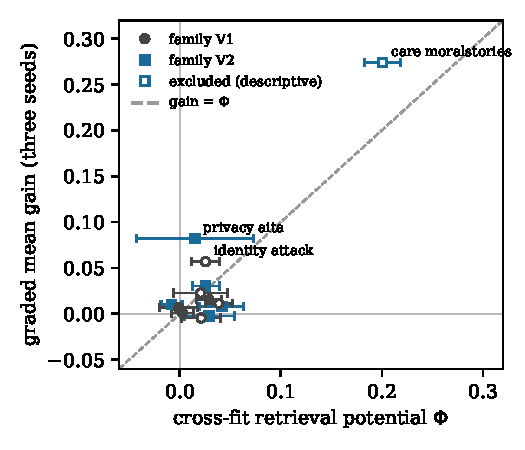
\includegraphics[width=0.72\columnwidth]{fig_gain_vs_phi.pdf}
  \caption{Graded mean gain against the cross-fit retrieval potential $\Phi$,
  thirteen units, fold-SD error bars. One large-$\Phi$ unit sits on the unit
  line; the rest sit at the instrument's noise floor. The correlation is
  Pearson $0.91$ at slope $1.3$, and the rank correlation is $0.22$.}
  \label{fig:phi}
\end{figure}

The post-hoc study asked what does order the magnitude. Three candidates
fail: the published reliability weights of the source encoders (tested as
V1's secondary bar), classification headroom (Spearman $0.181$ across the
thirteen units), and single-split retrieval headroom refined by
cross-fitting, which made the rank correlation worse ($0.352$ to $0.220$).
The quantity that succeeds in kind is the read metric's own retrieval
headroom: $\Phi=\mathrm{xfit}(R_C-A)$, where $R_C$ is 1-NN label accuracy
under $d_C$ on calibration data. Against $\Phi$ the graded gains lie near
the unit line (Pearson $0.908$, slope $1.30$; Figure~\ref{fig:phi}), and the
identification is close to definitional once stated: with the oracle ceiling
at $1$ and $k$ near-global, the graded gain is the grading split's retrieval
headroom under the frozen read.

Why then did two preregistrations fail? Because $\Phi$ cannot be estimated
in advance at natural sizes. The fold-level standard deviation of $\Phi$ is
$0.011$--$0.058$ across units, and ten of thirteen measured gains are below
$0.06$: the effects sit at the noise floor of the only instrument the
consumer has before grading. The one unit whose $\Phi$ stands eleven
standard deviations from zero is forecast correctly ($0.201\pm0.018$
predicted, $0.274$ measured). Three units additionally show
calibration-to-grading shift larger than their fold noise, so noise is not
the only failure mode. A sealable forecast would need either engineered
large-$\Phi$ units or calibration corpora an order of magnitude larger, and
we record that requirement rather than attempt a third seal on the present
pool.

The finding is worth stating in consumer-relative terms, because it is the
same shape as the phenomenon it measures. What retrieval is worth depends on
who reads the results; we add that how much it is worth is, at practical
sizes, invisible to the reader's own calibration channel. The two failed
seals are the evidence for that sentence, and we regard them as load-bearing
results rather than mishaps.

\section{Related work}

Metric learning, Mahalanobis and local variants, and trained rerankers are
long established; our reranker is not learned and our claim is not a better
reranker. Position-dependent Riemannian metrics from auxiliary information
were developed for exploratory analysis in the learning-metrics program
\cite{kaski2001,peltonen2004}, and NeRV made embedding quality explicitly
relative to a user's precision-recall cost \cite{venna2010}; our $P_C$ is
read off a deployed consumer rather than built from labels at embed time,
and where the consumer is itself a label probe the constructions nearly
coincide. Task-aware and decision-focused pipelines optimize models for
downstream decisions \cite{elmachtoub2022}; sensor-selection and
value-of-information literatures optimize weighted-trace objectives
\cite{joshiboyd2009}. We do not offer a better metric, reranker, or
selection rule. We offer the measurement: the conditional dissociation with
both arms sealed, two preregistered failures reported as executed, and the
identification of the magnitude with a potential the consumer cannot
estimate in advance.

\section{Scope and limitations}

One embedding family per phase, linear probes, top-1 label prediction, and
$k=50$ candidate generation whose ceiling never binds. The corpora are
English moral text and newsgroups; the cross-lingual arm covers
machine-translated Spanish and French databases only, and its stronger
invariance claim is refuted above. The distillation rule ties three units to
validated domain encoders; the rest use direct labels. All limits push in
the same direction: they narrow the settings in which we have measured the
law, not the honesty of the failures. In our controlled tests nothing
suggested the dissociation appears without measured misalignment, and we
claim nothing about that regime.

\section*{Reproducibility}

Every number above is read from committed, hashed records in the campaign
repository (sealed preregistrations, graded verdict JSONs, post-mortems, and
the determinant study), and the figure regenerates from them by script. The
two sealed families' verdicts are immutable; the repository's evidence
discipline file describes the seal and amendment rules.

\begin{thebibliography}{9}
\bibitem{kaski2001} S.~Kaski, J.~Sinkkonen, and J.~Peltonen,
``Bankruptcy analysis with self-organizing maps in learning metrics,''
\emph{IEEE Trans. Neural Networks}, vol.~12, 2001. % verify vol/pages on final
\bibitem{peltonen2004} J.~Peltonen, A.~Klami, and S.~Kaski,
``Improved learning of Riemannian metrics for exploratory analysis,''
\emph{Neural Networks}, vol.~17, 2004. % verify vol/pages on final
\bibitem{venna2010} J.~Venna, J.~Peltonen, K.~Nybo, H.~Aidos, and S.~Kaski,
``Information retrieval perspective to nonlinear dimensionality reduction for
data visualization,'' \emph{JMLR}, vol.~11, pp.~451--490, 2010.
\bibitem{elmachtoub2022} A.~N.~Elmachtoub and P.~Grigas, ``Smart `predict,
then optimize','' \emph{Management Science}, vol.~68, no.~1, 2022. % verify pages on final
\bibitem{joshiboyd2009} S.~Joshi and S.~Boyd, ``Sensor selection via convex
optimization,'' \emph{IEEE Trans. Signal Processing}, vol.~57, no.~2, 2009. % verify pages on final
\end{thebibliography}

\end{document}
